    \documentclass[12pt,a4paper]{article}
%DIF LATEXDIFF DIFFERENCE FILE
%DIF DEL submission1.tex   Wed Mar 26 11:15:42 2025
%DIF ADD paper.tex         Mon Apr  7 10:09:40 2025
    % Packages
\usepackage{amsfonts}
\usepackage{amsmath}
\usepackage{amssymb}
\usepackage[hidelinks]{hyperref}
\usepackage{cleveref}
\usepackage{graphicx}
\usepackage[round]{natbib}
\usepackage{float,soul}
\usepackage{tikz}
\usepackage{caption}
\usepackage{tabularx}
\usepackage{xr}  % external document -- for supplements

\captionsetup[figure]{labelfont=bf,font=footnotesize}
\captionsetup[table]{labelfont=bf,font=footnotesize}

% Figure placement
\makeatletter
\def\fps@figure{tb}
\makeatother

% Newcommands
\DeclareMathSymbol{\shortminus}{\mathbin}{AMSa}{"39}  % useful for suffixes
\newcommand{\Ex}{\mathbb{E}}
\newcommand{\Var}{\mathrm{Var}}
\newcommand{\HW}{\mathrm{HW}}
\newcommand{\Bin}{\text{Binomial}}
\newcommand{\Uniform}{\text{Uniform}}
%\newcommand{\Normal}{\text{Normal}}
\newcommand{\Normal}{\mathcal{N}}
\newcommand{\Beta}{\text{Beta}}
\newcommand{\Exp}{\text{Exponential}}
\newcommand{\Gam}{\text{Gamma}}
\newcommand{\Bfun}{\mathrm{B}}
\newcommand{\eps}{\epsilon}
\newcommand{\logit}{\mathop{\mathrm{logit}}}
\newcommand{\Vx}{\mathcal{V}}



    \usepackage[margin=1in]{geometry}
    \usepackage{authblk}
%DIF 5a5-6
    \usepackage{lineno} %DIF > 
    \linenumbers %DIF > 
%DIF -------
    \externaldocument[s-]{supp}
 %DIF > 
     %DIF > 
%DIF PREAMBLE EXTENSION ADDED BY LATEXDIFF
%DIF UNDERLINE PREAMBLE %DIF PREAMBLE
\RequirePackage[normalem]{ulem} %DIF PREAMBLE
\RequirePackage{color}\definecolor{RED}{rgb}{1,0,0}\definecolor{BLUE}{rgb}{0,0,1} %DIF PREAMBLE
\providecommand{\DIFadd}[1]{{\protect\color{blue}\uwave{#1}}} %DIF PREAMBLE
\providecommand{\DIFdel}[1]{{\protect\color{red}\sout{#1}}}                      %DIF PREAMBLE
%DIF SAFE PREAMBLE %DIF PREAMBLE
\providecommand{\DIFaddbegin}{} %DIF PREAMBLE
\providecommand{\DIFaddend}{} %DIF PREAMBLE
\providecommand{\DIFdelbegin}{} %DIF PREAMBLE
\providecommand{\DIFdelend}{} %DIF PREAMBLE
\providecommand{\DIFmodbegin}{} %DIF PREAMBLE
\providecommand{\DIFmodend}{} %DIF PREAMBLE
%DIF FLOATSAFE PREAMBLE %DIF PREAMBLE
\providecommand{\DIFaddFL}[1]{\DIFadd{#1}} %DIF PREAMBLE
\providecommand{\DIFdelFL}[1]{\DIFdel{#1}} %DIF PREAMBLE
\providecommand{\DIFaddbeginFL}{} %DIF PREAMBLE
\providecommand{\DIFaddendFL}{} %DIF PREAMBLE
\providecommand{\DIFdelbeginFL}{} %DIF PREAMBLE
\providecommand{\DIFdelendFL}{} %DIF PREAMBLE
%DIF LISTINGS PREAMBLE %DIF PREAMBLE
\RequirePackage{listings} %DIF PREAMBLE
\RequirePackage{color} %DIF PREAMBLE
\lstdefinelanguage{DIFcode}{ %DIF PREAMBLE
%DIF DIFCODE_UNDERLINE %DIF PREAMBLE
  moredelim=[il][\color{red}\sout]{\%DIF\ <\ }, %DIF PREAMBLE
  moredelim=[il][\color{blue}\uwave]{\%DIF\ >\ } %DIF PREAMBLE
} %DIF PREAMBLE
\lstdefinestyle{DIFverbatimstyle}{ %DIF PREAMBLE
	language=DIFcode, %DIF PREAMBLE
	basicstyle=\ttfamily, %DIF PREAMBLE
	columns=fullflexible, %DIF PREAMBLE
	keepspaces=true %DIF PREAMBLE
} %DIF PREAMBLE
\lstnewenvironment{DIFverbatim}{\lstset{style=DIFverbatimstyle}}{} %DIF PREAMBLE
\lstnewenvironment{DIFverbatim*}{\lstset{style=DIFverbatimstyle,showspaces=true}}{} %DIF PREAMBLE
%DIF END PREAMBLE EXTENSION ADDED BY LATEXDIFF

\begin{document}
    \title{Autopolyploid establishment through polygenic adaptation}
    %\author[1]{Arthur Zwaenepoel\thanks{arthur.zwaenepoel@uantwerpen.be}}
    %\affil[1]{\footnotesize Department of Biology, University of Antwerp, 2020 Antwerp, Belgium}
    \author{}
    \date{\vspace{-5ex}}
    \maketitle
    \begin{abstract}
    We define the infinitesimal model of quantitative genetics \DIFdelbegin \DIFdel{(}\textit{\DIFdel{sensu}}
    %DIFAUXCMD
\DIFdel{\mbox{%DIFAUXCMD
\cite{barton2017}}\hspace{0pt}%DIFAUXCMD
) }\DIFdelend for the inheritance
        of an additive quantitative trait in a mixed-ploidy population consisting
        of diploid, triploid and autotetraploid individuals producing haploid and
        diploid gametes.
        We implement efficient simulation methods and use these to study the
        quantitative genetics of mixed-ploidy populations and the establishment of
        autotetraploids in a new habitat.
        We show that\DIFdelbegin \DIFdel{for rare }\DIFdelend \DIFaddbegin \DIFadd{, when }\DIFaddend migration from the source population \DIFaddbegin \DIFadd{is rare}\DIFaddend ,
        autotetraploids are more likely to \DIFdelbegin \DIFdel{found a successful
    population }\DIFdelend \DIFaddbegin \DIFadd{establish in the new habitat 
        }\DIFaddend than diploids under a very broad range of conditions, but that this
        is unlikely to sufficiently counter the scarcity of tetraploid founders
        when the source is predominantly diploid.
        We assess in more detail how minority cytotype exclusion interacts with
        migration load in the establishment process and evaluate the impact of
        additional sources of prezygotic isolation, specifically selfing and
        assortative mating, on the relative establishment probabilities of the
        different cytotypes \DIFaddbegin \DIFadd{in the presence of maladaptive migration}\DIFaddend .
        In the discussion we consider how inbreeding depression may impact our
        findings.

        \textbf{Keywords:} polyploidy, adaptation, establishment, inbreeding,
        quantitative genetics 
    \end{abstract}

    \section*{Introduction}

    %DIF <  Should connect more with literature and concepts of isolating mechanisms pre
%DIF <  vs. postzygotic isolation, and reinforcement etc. (see e.g. Parvathy &
%DIF <  Himani's paper introduction)
\DIFdelbegin %DIFDELCMD < 

%DIFDELCMD < %%%
\DIFdelend Many plant species exhibit ploidy variation
    \citep{levin2002,soltis2007,rice2015}, and many of these \textit{mixed-ploidy}
    species have populations in which different cytotypes coexist or form contact
    zones \citep{kolar2017}.
    How such mixed-ploidy populations emerge and are maintained has proven somewhat
    challenging to understand.

    Consider for instance a randomly mating diploid population.
    Under the commonly accepted view that new polyploid plants are mostly formed
    through the union of unreduced gametes
    \citep{bretagnolle1995,herben2016,kreiner2017b}, a new tetraploid individual
    originating by a chance encounter of two unreduced diploid gametes (an event
    occurring at an appreciable rate; \cite{kreiner2017}) is highly unlikely to
    establish a stable tetraploid subpopulation, as most of its gametes will end up
    in unfit hybrids of odd ploidy level (a phenomenon referred to as `triploid
    block', see \cite{ramsey1998,kohler2010,brown2024}).
    This \DIFdelbegin \DIFdel{negative }\DIFdelend \DIFaddbegin \DIFadd{positive }\DIFaddend frequency dependence effect \DIFaddbegin \DIFadd{in mixed-ploidy populations }\DIFaddend is
    commonly referred to as \textit{minority cytotype exclusion} (MCE), after
    \cite{levin1975}.
    It is well-appreciated that, as a consequence of MCE, the rate of unreduced
    gamete formation needs to be extraordinarily high for tetraploids to establish
    \DIFaddbegin \DIFadd{a stable subpopulation }\DIFaddend in a large random mating \DIFdelbegin \DIFdel{initially diploid population }\DIFdelend \DIFaddbegin \DIFadd{population initially dominated
    by diploids }\DIFaddend (\cite{felber1997}, see also \cref{s-sec:det}).

    Hence, to explain the widespread occurrence of mixed-ploidy populations,
    additional factors besides the continuous formation of polyploids through the
    union of unreduced gametes need to be considered.
    Firstly, chance establishment of tetraploids through drift could occur.
    Indeed, the problem is somewhat analogous to the spread of underdominant
    chromosomal rearrangements, where local establishment through genetic drift and
    subsequent spreading in a subdivided population \DIFdelbegin \DIFdel{through }\DIFdelend \DIFaddbegin \DIFadd{by means of }\DIFaddend local extinction
    and recolonization \DIFdelbegin \DIFdel{dynamics }\DIFdelend has been suggested as a plausible model \citep{lande1985}.
    However, MCE is quite strong \DIFdelbegin \DIFdel{in randomly matingmixed-ploidy populations}\DIFdelend \DIFaddbegin \DIFadd{under random mating}\DIFaddend , and the population size has
    to be very small for local tetraploid establishment to occur at an appreciable
    rate (\cite{rausch2005}, see also \cref{s-sec:mchain}).
    Secondly, any form of \textit{prezygotic isolation} between cytotypes could
    promote establishment of polyploid cytotypes by alleviating MCE.
    Particularly relevant are assortative mating by cytotype  (for instance through
    phenological differences across cytotypes, or differences in pollinators;
    \DIFdelbegin \DIFdel{\mbox{%DIFAUXCMD
\cite{kolar2017}}\hspace{0pt}%DIFAUXCMD
}\DIFdelend \DIFaddbegin \DIFadd{\mbox{%DIFAUXCMD
\cite{husband2004,kolar2017}}\hspace{0pt}%DIFAUXCMD
}\DIFaddend ), self-fertilization \citep{rausch2005,novikova2023}, 
    \DIFdelbegin \DIFdel{and
}\DIFdelend localized dispersal \citep{baack2005,kolar2017} \DIFaddbegin \DIFadd{and asexual reproduction
    \mbox{%DIFAUXCMD
\citep{vandrunen2022}}\hspace{0pt}%DIFAUXCMD
}\DIFaddend .
    Finally, selection may be invoked to explain the establishment of polyploids.
    Tetraploids may have higher relative fitness than their diploid counterparts
    due to reduced inbreeding depression
    \DIFdelbegin \DIFdel{\mbox{%DIFAUXCMD
\citep{ronfort1999,otto2000}}\hspace{0pt}%DIFAUXCMD
}\DIFdelend \DIFaddbegin \DIFadd{\mbox{%DIFAUXCMD
\citep{husband1997,ronfort1999,otto2000,husband2004,husband2008,clo2022b}}\hspace{0pt}%DIFAUXCMD
}\DIFaddend , or due to being
    better adapted to (changing) environmental conditions \citep{vandepeer2021}. 
    \DIFdelbegin %DIFDELCMD < 

%DIFDELCMD < %%%
\DIFdel{None }\DIFdelend \DIFaddbegin \DIFadd{However, none }\DIFaddend of these factors is likely to explain by itself the establishment
    of polyploids, and the consensus in the field appears to be that some mix of
    the above is required to explain the occurrence of mixed-ploidy populations in
    nature \citep{kolar2017,mortier2024}.
\DIFdelbegin \DIFdel{In particular, polyploids
    are thought to establish mainly in novel, unoccupied
habitats where they evade MCE (for instance at range edges, or after local
extinction due to environmental change) \mbox{%DIFAUXCMD
\citep{griswold2021}}\hspace{0pt}%DIFAUXCMD
}\DIFdelend \DIFaddbegin 

    \DIFadd{Many empirical studies of mixed-ploidy populations find that polyploids
    established in peripheral habitats at the edge of a species' range (reviewed in
    \mbox{%DIFAUXCMD
\cite{griswold2021}}\hspace{0pt}%DIFAUXCMD
), and this is in accord with large scale biogeographical
    patterns \mbox{%DIFAUXCMD
\citep{rice2019}}\hspace{0pt}%DIFAUXCMD
.
    This raises the question: which aspects of the process of adaptation to marginal
    habitats could promote the establishment of polyploid populations?
    In a peripheral habitat, a new polyploid population may be more likely to reach
    an appreciable size as it evades to some extent the negative effects of MCE
    \mbox{%DIFAUXCMD
\citep{levin1975}}\hspace{0pt}%DIFAUXCMD
}\DIFaddend .
    However, \DIFaddbegin \DIFadd{at the same time, }\DIFaddend such peripheral habitats are likely to present
    adaptive challenges to establishment
    \DIFdelbegin \DIFdel{\mbox{%DIFAUXCMD
\citep{kawecki2008adaptation}}\hspace{0pt}%DIFAUXCMD
}\DIFdelend \DIFaddbegin \DIFadd{\mbox{%DIFAUXCMD
\citep{kawecki2008adaptation,sachdeva2022b}}\hspace{0pt}%DIFAUXCMD
}\DIFaddend , and if polyploids are able to
    colonize such habitats at an appreciable rate, they must somehow be better
    adapted to local conditions, or more able to adapt to those conditions despite
    inbreeding and maladaptive migration, compared to diploids.
\DIFdelbegin \DIFdel{Indeed, when the source population is dominated by diploids, the probability
that a migrant individual is tetraploid will be very small ($\sim u^2$, where
$u$ is the probability that a diploid produces an unreduced gamete in meiosis),
    so that tetraploids need a substantial advantage during
    colonization if they
are to establish before diploids do}\DIFdelend \DIFaddbegin 

    \DIFadd{More often than not, local adaptation is polygenic in nature
    \mbox{%DIFAUXCMD
\citep{pritchard2010,barghi2020,bomblies2022}}\hspace{0pt}%DIFAUXCMD
, involving many weakly selected
    variants across the genome, and adaptation during polyploid establishment
    in a marginal habitat is unlikely to present an exception.
    Recent studies on local adaptation in autopolyploids indeed tend to find a
    polygenic basis of adaptation \mbox{%DIFAUXCMD
\citep{bohutinska2021,konevcna2021,konevcna2022}}\hspace{0pt}%DIFAUXCMD
,
    however it is not clear how observed adaptive differentiation in established
    tetraploid populations relates to adaptation that may have occurred during
    initial establishment}\DIFaddend .

    While there have been substantial modeling efforts aimed at understanding
    autotetraploid establishment within diploid populations \citep{levin1975,
    felber1991, felber1997, rausch2005, oswald2011, clo2022c}, the problem of
    polyploid establishment in peripheral habitats remains largely unaddressed
    (but see \cite{griswold2021}),
    despite its centrality to verbal arguments about the establishment of
    polyploids in natural populations \citep{kolar2017, vandepeer2021, clo2022d}.

    Here we develop a model for the establishment of a mixed-ploidy population in a
    novel, unoccupied habitat based on \cite{barton2018}.
    In order to establish in the novel habitat, the population has to adapt to
    local environmental conditions.
    We assume fitness is determined by directional selection on a single polygenic
    trait, which can be interpreted as log fitness at low density in the new
    habitat.
    As in \cite{barton2018}, we assume the trait follows the infinitesimal
    model (\textit{sensu} \cite{barton2017}, i.e. the `Gaussian descendants'
    infinitesimal model \citep{turelli2017}).
    We extend the infinitesimal model, and the approach for exact simulation of
    trait evolution under the infinitesimal model, to mixed-ploidy populations.
    This is a first contribution of the present paper.
    We then use simulations to study tetraploid establishment, both from single
    migrants and under continuous migration from a predominantly diploid source
    population, examining the effects of autopolyploid genetics,
    maladaptive migration, selfing and assortative mating on the probability that
    autotetraploids establish in the novel habitat.


    \section*{Model and Methods}

    \begin{table}[t]
    \caption{Glossary of the notation used in the main text.
    } \label{tbl:glossary}
    \centering
    \small
    \begin{tabularx}{\linewidth}{lX}
    \cline{1-2}
    \textbf{notation}   & \textbf{description}   \\ \cline{1-2}
    $N$ & total population size\\
    $N_k$ & population size of the $k$-ploid cytotype \\
    $\pi_k$ & deterministic equilibrium frequency of the $k$-ploid cytotype \\
    $u$ & probability of unreduced gamete formation ($u=u_{22}=1-u_{42}$)\\
    $v$ & probability that a triploid produces a haploid/diploid gamete
      ($v=u_{31}=u_{32}$)\\
    $m$ & expected number of migrants per generation arriving in the new habitat \\
    $z_i$ & trait value of individual $i$ \\
    $c_i$ & ploidy level of individual $i$ \\
    $g_i$ & ploidy level of gamete produced by individual $i$ in a particular cross\\
    $V$ & segregation variance in the reference diploid population \\
    $V_{i,k}$ & gametic segregation variance associated with the production of a
      $k$-ploid gamete by individual $i$ \\
    $\Vx_k$ & genetic variance associated with a haploid genome in the $k$-ploid
      reference population (i.e. a $k$-ploid non-inbred population at HWLE) \\
    $\beta_{k}$ & scaling factor for allelic effects in $k$-ploids \\
    $F_i$ & inbreeding coefficient in individual $i$ \\
    $\Phi_{ij}$ & coancestry coefficient for individuals $i$ and $j$ \\
    $\alpha_k$ & probability that the two genes at a locus in a diploid gamete
      formed by a $k$-ploid individual descend from the same parental gene copy\\
    $\gamma$ & strength of directional selection in the new habitat\\
    $\theta$ & trait value beyond which the growth rate becomes positive in the new
        habitat \\ 
    $w_{ij}$ & fitness of parental pair $(i,j)$ \DIFaddbeginFL \DIFaddFL{(expected fitness of
        offspring of pair $(i,j)$)}\DIFaddendFL \\
    $w_{ij}^{kl}$ & expected fitness of offspring \DIFdelbeginFL \DIFdelFL{from }\DIFdelendFL \DIFaddbeginFL \DIFaddFL{of }\DIFaddendFL parental pair $(i,j)$ when
    $i$ contributes a $k$-ploid gamete and $j$ contributes a $l$-ploid gamete \\
    $\sigma_k$ & rate of self-fertilization in $k$-ploids \\
    $\rho_k$ & probability of assortative mating in $k$-ploids \\
    \cline{1-2}
    \end{tabularx}%
    \end{table}

    \subsection*{Mixed-ploidy population model}

    Our notation is summarized in \cref{tbl:glossary}.
    We consider a mixed-ploidy population of size $N$ consisting of $N_2$ diploid,
    $N_3$ triploid and $N_4=N-N_2-N_3$ tetraploid individuals.
    We assume an individual of ploidy level $k$ forms haploid and diploid gametes
    with proportions $u_{k1}$ and $u_{k2}$, as well as a proportion
    $1-u_{k1}-u_{k2}$ inviable (e.g. aneuploid or polyploid) gametes.
    The (relative) fecundity of a $k$-ploid individual is hence $u_{k1} + u_{k2}$.
    Unless stated otherwise, we will assume 
    \begin{equation}
        \begin{pmatrix} 
        u_{21} & u_{22} \\ 
        u_{31} & u_{32} \\ 
        u_{41} & u_{42} 
        \end{pmatrix} =
        \begin{pmatrix} 
        1-u & u \\
        v & v \\
        0 & 1-u
        \end{pmatrix} \label{eq:U}
    \end{equation}
    where $u$ is referred to as the proportion of unreduced gametes, and $2v$ is
    the proportion of euploid gametes produced by a triploid individual.
    \DIFaddbegin \DIFadd{The rate of unreduced gamete production is hence fixed across individuals, and
    is assumed to be the same in diploids and tetraploids.
}\DIFaddend 

    When two individuals mate, we assume they produce gametes according to their
    ploidy level (\cref{eq:U}), which randomly combine to produce offspring (which
    may be inviable if one of the contributing gametes is inviable).
    Intrinsic fitness disadvantages associated with particular zygotic ploidy
    levels or cross types (e.g. modeling phenomena such as `triploid block') can be
    straighforwardly included at this level.
    An analysis of a deterministic model (i.e. where $N \rightarrow \infty$) for
    the cytotype dynamics and equilibrium cytotype composition under random mating
    is included in \cref{s-sec:det} (see also \cite{felber1997,kauai2024}).
    The stochastic version for finite and constant $N$ is analyzed briefly in
    \cref{s-sec:mchain}.

    \subsection*{Infinitesimal model}

    \paragraph*{The basic infinitesimal model.}

    Consider a population which expresses a quantitative trait determined by a
    large number of additive loci of small effect.
    The infinitesimal model approximates the inheritance of such a trait by
    assuming that the trait value $Z_{ij}$ of a random offspring from parents with
    trait values $z_i$ and $z_j$ follows a Gaussian distribution with mean equal to
    the midparent value and variance which is independent of the mean:
      \begin{align}
      Z_{ij} \sim \Normal\left(\frac{z_i + z_j}{2}, V_{ij}\right)
      \label{eq:inf}
      \end{align}
    Here, $V_{ij}$ is referred to as the \textit{segregation variance} in family
    $(i,j)$.
    This is the variation generated among offspring from the same parental pair due
    to random Mendelian segregation in meiosis.
    This approximation can be justified as arising from the limit where the number
    of loci determining the trait tends to infinity \citep{barton2017}.

    An alternative, and for our purposes useful, way to characterize the model
    is to write $Z_{ij} = Y_i + Y_j$, where $Y_i$ and $Y_j$
    are independent Gaussian random variables $Y_i \sim \Normal\left(\frac{z_i}{2},
    V_i\right)$ (and similarly for $Y_j$).
    We refer to $Y_i$ as the (random) \textit{gametic value} of individual $i$, and
    to $V_i$ as the \textit{gametic segregation variance} of individual $i$.
    This formulation is helpful in that it highlights that Mendelian segregation
    occurs independently in both parents to produce gametes, which then combine
    additively to determine the offspring trait value.
    This model applies readily to an autopolyploid population expressing a trait
    with infinitesimal genetics.
    However, the segregation variance will be determined by the details of
    tetraploid meiosis, which differ from those of diploid meiosis (see below).

    In a finite population, the segregation variance will decay over time as the
    population becomes more inbred (Mendelian segregation at homozygous loci does
    not generate any variation).
    When $F_i$ is the inbreeding coefficient relative to some ancestral reference
    population with gametic segregation variance $V$ (i.e. the probability that two
    genes at a locus in individual $i$ sampled without replacement are identical by
    descent), the gametic segregation variance of individual $i$ will be
    $V_i = (1-F_i)V$.
    This holds for both diploids and tetraploids (\cref{s-sec:tetinbred}, also
    \cite{moody1993}). 

    \paragraph{Scaling of traits across ploidy levels.}

    If we would naively assume that the allelic effects underlying an additive
    trait are identical across ploidy levels, 
    a tetraploid offspring from a cross between two diploids would have, on average,
    a trait value which is the sum of the parental trait values.
    This is not likely to reflect biological reality: tetraploids do not tend to
    have, for instance, twice the size of their diploid progenitors on average
    \DIFaddbegin \DIFadd{(e.g. \mbox{%DIFAUXCMD
\cite{porturas2019}}\hspace{0pt}%DIFAUXCMD
)}\DIFaddend .
    Furthermore, the genetic variance at Hardy-Weinberg and linkage equilibrium
    (HWLE) in a large non-inbred tetraploid population will be twice that of their
    diploid counterparts under such assumptions, which is similarly unrealistic
    \citep{clo2022}.

    In order to account for this, we introduce a scaling factor $\beta_k$,
    accounting for the effects of polyploidization \textit{per se} on trait
    expression in $k$-ploids.
    To introduce and interpret this parameter, we consider an $L$-locus additive
    model, with two alleles (0 and 1) at each locus.
    For a $k$-ploid individual, let $X_{i,j}$ be the allele at homolog $j$ of locus
    $i$.
    We assume the trait value is determined by
    \begin{equation}
      z = \sum_{i=1}^L\sum_{j=1}^k a_{i,k} X_{i,j}
    \end{equation}
    Where $a_{i,k}$ is the allelic effect of the 1 allele at locus $i$ in
    $k$-ploids.
    The genetic variance at HWLE in $k$-ploids ($\tilde{V}_{z,k}$) will then be
    \begin{equation}
      \tilde{V}_{z,k} = k\sum_{i=1}^L a_{i,k}^2 p_iq_i = k\Vx_{k}
    \end{equation}
    where we refer to $\Vx_{k}$ as the variance associated with a haploid genome in
    $k$-ploids at HWLE.
    If we now assume $a_{i,k} = \beta_k a_{i,2}$, i.e. allelic effects in $k$-ploids
    are as in diploids, but scaled homogeneously by a factor $\beta_k$, and assume
    equal allele frequencies in the different cytotypes, we will have
    \begin{equation}
      \frac{\tilde{V}_{z,k}}{\tilde{V}_{z,2}} 
      = \frac{k\Vx_{k}}{2\Vx_{2}} = \frac{k}{2} \beta_{k}^2
    \end{equation}
    Note that by definition $\beta_2=1$.
    Under the infinitesimal model (where $a_{i,2} \rightarrow 0$ as $L\rightarrow
    \infty$), we have $\tilde{V}_{z,2} = 2\Vx_{2} = 2V$ \citep{barton2017}, where
    $V$ is the segregation variance in the diploid population.
    Hence, in the infinitesimal limit we have $\Vx_{k} = \beta_k^2 \Vx_{2} =
    \beta_k^2 V$.


    \paragraph{Mixed-ploidy infinitesimal model.}

    We can extend the infinitesimal model to the mixed-ploidy case, assuming that the
    gametic value, on the diploid trait scale, associated with a $k$-ploid gamete ($k
    \in \{1,2\}$) from individual $i$ of ploidy level $c_i \in \{2,3,4\}$ is a
    Gaussian random variable $Y_{i,k}$ with distribution
    \begin{equation}
        Y_{i,k} \sim \Normal\left(\frac{k}{c_i}\frac{z_i}{\beta_{c_i}}, V_{i,k}\right)
        \label{eq:gamete}
    \end{equation}
    where $V_{i,k}$ is the gametic segregation variance associated with the
    production of a $k$-ploid gamete by individual $i$ (see below).
    The trait value of an individual originating from the union of a $k$-ploid
    gamete of individual $i$ and an $l$-ploid gamete from individual $j$ is then
      $$Z_{ij}^{kl} = \beta_{k+l}\left(Y_{i,k} + Y_{j,l}\right)$$
    i.e., $Z_{ij}^{kl}$ is a Gaussian random variate with distribution
        \DIFdelbegin \begin{displaymath}
  \DIFdel{Z_{ij}^{kl} \sim \Normal\left(
    \beta_{k+l} \left(
          \frac{k}{c_i}\frac{z_i}{\beta_{c_i}} 
        + \frac{l}{c_j}\frac{z_j}{\beta_{c_j}}\right), 
    \beta_{k+l}^2 (V_{i,k} + V_{j,l})\right)
   %DIFDELCMD < \label{eq:oneline}%%%
}\end{displaymath}%DIFAUXCMD
\DIFdelend \DIFaddbegin \DIFadd{$Z_{ij}^{kl} \sim \Normal\left(\overline{z_{ij}^{kl}},
        V_{ij}^{kl}\right)$
    where
    }\begin{align}
        \DIFadd{\overline{z_{ij}^{kl}} }&\DIFadd{= \beta_{k+l} \left(
              \frac{k}{c_i}\frac{z_i}{\beta_{c_i}} 
            + \frac{l}{c_j}\frac{z_j}{\beta_{c_j}}\right) \nonumber }\\
        \DIFadd{V_{ij}^{kl} }&\DIFadd{= \beta_{k+l}^2 (V_{i,k} + V_{j,l})
       \label{eq:oneline}
    }\end{align}\DIFaddend 

    The gametic segregation variance associated with the production of diploid
    gametes depends not only on the segregation variance in the base population
    ($V$) and the inbreeding coefficient ($F$), but also on the detailed
    assumptions of how the meiotic process takes place.
    Importantly however, the latter only affect the gametic segregation variance
    through the quantity $\alpha_k$, which is the probability that a $k$-ploid
    transmits two copies of the same homolog to a diploid gamete.
    Note that $\alpha_4$, the probability that a diploid gamete of a tetraploid
    individual carries two copies of the same homolog, is the probability of
    \textit{double reduction} (e.g. \cite{lynch1998} p.57), and is upper bounded by
    1/6 \citep{stift2008}.
    The value of $\alpha_2$ depends on the relative frequency of unreduced gamete
    formation through so-called \textit{first} and \textit{second division
    restitution} \citep{bretagnolle1995,storme2013}.
    We summarize the expressions for the gametic segregation variance in
    \cref{tbl:segvar}.
    Detailed derivations can be found in \cref{s-sec:segvar}.


    \begin{table}[t]
    \caption{Gametic segregation variance for haploid and diploid gametes produced
    by the three cytotypes in the mixed-ploidy model. $F_i$ is the inbreeding
    coefficient of individual $i$ (producing the gamete), whereas $\alpha_k$ is the
    probability that a diploid gamete from a $k$-ploid individual receives two
    copies of the same parental gene. We assume $\alpha_3 \le 1/4$ and
        $\alpha_4 \le 1/6$ (see \cref{s-sec:segvar}).
    } \label{tbl:segvar}
    \centering
    \small
    \begin{tabularx}{\linewidth}{XXX}
    \cline{1-3}
    \textbf{cytotype}   & \textbf{haploid gamete variance} & \textbf{diploid gamete
    variance}        \\ \cline{1-3} \\[-2.5ex]
    diploid    & $\frac{1}{2}(1-F_i)V$    & $2\alpha_2(1-F_i)V$  \\ \\[-2.5ex]
    triploid   & $\frac{2}{3}(1-F_i)V$     & $\frac{2}{3}(1 + 3\alpha_3)(1-F_i)V$ \\ \\[-2.5ex]
    tetraploid & --                      & $(1+2\alpha_4)(1-F_i)V$             \\
    \cline{1-3}
    \end{tabularx}%
    \end{table}

    Writing $\bar{z}_2$ for the mean trait value in the diploid subpopulation,
    \cref{eq:oneline} implies that a tetraploid offspring from a random diploid
    parental pair has an expected trait value equal to $\bar{z}_4 =
    2\beta_4\bar{z}_2$.
    This hence implies that $|\bar{z}_4| \ge |\bar{z}_2|$, with equality only when
    $\beta_4=1/2$ or $\bar{z}_2 = \bar{z}_4 = 0$. 
    In other words, when $\beta_4 > 1/2$, we would have for all but $\bar{z}_2 = 0$
    that newly formed tetraploids have more extreme phenotypes on average than
    their diploid parents.
    In our establishment model (see below), we shall therefore always consider 
    the case where $\bar{z}_2=0$ in the source population, and think of the trait
    value modeled as the deviation from the mean phenotype in the source
    population.

    The property that polyploid phenotypes are more extreme on average makes sense
    if we consider the underlying genetic model: if we assume the source population
    is at an equilibrium between mutation, drift and stabilizing selection,
    segregating genetic variants that affect the trait will be equally likely to
    have positive or negative allelic effects \citep{hayward2022}.
    At equilibrium, any diploid individual with trait value $z - \bar{z}_2 > 0$
    then carries an excess of variants with positive allelic effects on the trait,
    and this excess should be exaggerated in its polyploid offspring, which carry
    \textit{twice} the excess of their parent on average.
    In other words, the mixed-ploidy model is not `\DIFdelbegin \DIFdel{coordinate free}\DIFdelend \DIFaddbegin \DIFadd{coordinate-free}\DIFaddend ' as the basic
    infinitesimal model is: \cref{eq:oneline} only makes sense when the trait
    values that are modeled correspond to deviations from the mean values
    associated with an underlying equilibrium state.


    \paragraph{Recursions for inbreeding coefficients}

    We can simulate the mixed-ploidy infinitesimal model for a finite population
    through a straightforward extension of the approach outlined in
    \cite{barton2017}, provided we can efficiently track inbreeding and coancestry
    coefficients across the different ploidy levels.
    Denoting the parents of individual $i$ by $k$ and $l$, the recursion for the
    inbreeding coefficients in the mixed-ploidy case becomes
    \begin{align}
        F_i &= \Phi_{kl} & \text{if } & c_i = 2 \nonumber \\ 
        F_i &= \frac{1}{3}\left(F_k^\ast + 2\Phi_{kl}\right) & \text{if } 
            & c_i = 3, g_k = 2, g_l = 1 \nonumber \\ 
        F_i &= \frac{1}{3}\left(F_l^\ast + 2\Phi_{kl}\right) & \text{if } 
            & c_i = 3, g_k = 1, g_l = 2 \nonumber \\ 
        F_i &= \frac{1} 6 (F_k^\ast + F_l^\ast + 4\Phi_{kl}) & \text{if } & c_i = 4
    \end{align}
    where $F_k^\ast = \alpha_{c_k} + (1-\alpha_{c_k})F_k$ (\cref{s-sec:tetinbred}).
    The recursion for the coancestry coefficients is given by
    \begin{align}
        \Phi_{ii} &= \frac{1}{c_{i}} \left(1 + (c_i-1)F_i\right) \nonumber \\
        \Phi_{ij} &= \sum_k \sum_l P_{ik}P_{jl} \Phi_{kl} & i \ne j 
        \label{eq:coancestry}
    \end{align}
    where the sums are over individuals in the parental population, and where
    $P_{ik} \in \{0, \frac{1} 3, \frac{1} 2, \frac{2} 3, 1\}$ is the probability that a
    gene copy in \DIFaddbegin \DIFadd{individual }\DIFaddend $i$ is derived from parent $k$.

    \subsection*{Establishment model}

    Our model for the establishment of a population in an initially unoccupied
    habitat is based on \cite{barton2018}.
    We assume a large non-inbred `mainland' mixed-ploidy population at HWLE and
    cytotype equilibrium, with $\Ex[z] = 0$ irrespective of the cytotype.
    The equilibrium trait value distribution for the different cytotypes on the
    mainland is complicated in general, but a very accurate approximation (which we
    use throughout) is readily obtained for the case where $u$ is small (see
    \cref{s-sec:mixeq}).

    In generation $t$, $M(t)$ migrant individuals arrive on an island (the new
    habitat) joining $N^\ast(t)$ resident individuals, where $M(t)$ is Poisson
    distributed with mean $m$\DIFaddbegin \DIFadd{, and $N^\ast(0)=0$ unless stated otherwise}\DIFaddend . 
    The migrant individuals are assumed to be unrelated to the resident
    individuals.
    After migration \DIFdelbegin \DIFdel{in generation $t$, the }\DIFdelend \DIFaddbegin \DIFadd{there are }\DIFaddend $N(t) = N^\ast(t) + M(t)$ individuals \DIFaddbegin \DIFadd{on the island
    which }\DIFaddend reproduce sexually, and the offspring thus produced survives until the
    next generation with a probability determined by their trait value.
    \DIFaddbegin \DIFadd{Note that this corresponds to a life cycle where selection occurs before
    migration within a generation.
    }\DIFaddend In the basic model, random selfing is allowed (but see below for a model with
    self-incompatibility).
    We assume the trait is under directional selection, with fitness $w(z) =
    e^{\gamma(z - \theta)}$, where $\gamma$ is the intensity of directional
    selection and $\theta$ is the trait value for which the growth rate of the
    island population becomes positive.
    As the population becomes better adapted, eventually, some form of density
    regulation must limit its growth.
    We ignore density regulation throughout and focus on the initial establishment
    phase, defining establishment as reaching a population of size 100.

    Again following \cite{barton2018}, we simulate the model by first calculating
    the fitness of each parental pair $(i,j)$, which is the expected fitness of
    offspring of this pair
    \begin{equation}
      w_{ij}
        = \sum_{k=1}^2\sum_{l=1}^2 w_{ij}^{kl}
        = \sum_{k=1}^2\sum_{l=1}^2 u_{c_{i},k}u_{c_{j},l}
            \Ex\left[e^{\gamma(Z_{ij}^{kl} - \theta)}\right]
    \end{equation}
    The expectation on the right hand side can be calculated from \cref{eq:oneline}
    using the moment-generating function of the Gaussian\DIFdelbegin \DIFdel{.
}\DIFdelend \DIFaddbegin \DIFadd{, i.e.
    }\begin{equation}
        \DIFadd{\Ex\left[e^{\gamma(Z_{ij}^{kl} - \theta)}\right] 
        = e^{\gamma \left(\overline{z_{ij}^{kl}} -\theta\right) +
        \frac{\gamma^2}{2}
        V_{ij}^{kl}} 
        \label{eq:Ew}
    }\end{equation}
    \DIFaddend Having calculated the $w_{ij}$, the number of offspring surviving into the next
    generation is calculated as $N^\ast(t+1) = \sum_{i,j}w_{ij}/N(t)$.
    Next, $N^\ast(t+1)$ offspring individuals are \DIFdelbegin \DIFdel{sampled }\DIFdelend \DIFaddbegin \DIFadd{obtained }\DIFaddend by sampling parental
    pairs and gametes proportional to $w_{ij}^{kl}$, and sampling a trait value
    \DIFdelbegin \DIFdel{in accordance with }%DIFDELCMD < \cref{eq:oneline}%%%
\DIFdelend \DIFaddbegin \DIFadd{from a Gaussian distribution with mean $\overline{z_{ij}^{kl}} + \gamma
    V_{ij}^{kl}$ and variance $V_{ij}^{kl}$}\DIFaddend . 

    \subsection*{Self-fertilization and assortative mating}

    We model partial self-fertilization by assuming that a proportion
    $\sigma_{c_i}$ of the ovules of individual $i$ with ploidy level $c_i$ are
    fertilized by self-pollen, while the remaining proportion $1-\sigma_{c_i}$ are
    fertilized by randomly sampled pollen (which may be self-pollen with
    probability $1/N$). 
    That is, the expected number of offspring from individual $i$ as mother
    surviving after selection is
    \begin{equation}
    \Ex[w_i] = \sigma_{c_i} w_{ii} +
      (1-\sigma_{c_i})\left[\frac{1}{N}\sum_{j=1}^N w_{ij}\right]
    \end{equation}
    We hence assume no pollen limitation (all outcrossing ovules are fertilized),
    and no pollen discounting (the probability of being a father is unaffected by
    an individual's selfing rate).
    When modeling self-incompatibility, we assume there is no intrinsic
    disadvantage to self-incompatibility, except when there is only a single
    individual in the population, i.e.
    \begin{equation}
    \Ex[w_i] = \begin{cases}
        \frac{1}{N-1}\sum_{j \ne i }w_{ij} & \text{if } N > 1\\ 
        0 & \text{if } N=1 \end{cases}
    \end{equation}

    We model assortative mating by ploidy level in a similar way, assuming that a
    fraction $\rho_{c_i}$ of the ovules of individual $i$ are fertilized by pollen
    sampled from the $c_i$-ploid portion of the population, while a fraction
    $1-\rho_{c_i}$ is fertilized by pollen randomly sampled from the entire
    population.
    \begin{equation}
    \Ex[w_i] = \rho_{c_i} \frac{1}{N_{c_{i}}} \sum_{j=1}^N \delta_{c_i,c_j}w_{ij}
     + (1-\rho_{c_i})
    \left[\frac{1}{N}\sum_{j=1}^N w_{ij}\right]
    \end{equation}
    Where $\delta_{x,y}$ is the Kronecker delta function.

    \subsection*{Implementation and availability}

    Individual-based simulations for the mixed-ploidy infinitesimal model were
    implemented in Julia \citep{julia}.
    Documented code and simulation notebooks are available at \url{[anonymized]}.
%DIF > \url{https://github.com/arzwa/InfGenetics}.

\section*{Results}

The results section is organized as follows: first we verify the correctness
and accuracy of the infinitesimal model for mixed-ploidy populations by
comparison against simulations of a model with finitely many loci.
Next we assess how autotetraploid genetics and different assumptions on the
genetic variance of neotetraploids affect the probability of tetraploid
establishment in a marginal habitat relative to diploid establishment, starting
from a single maladapted migrant individual.
We then study how continuous migration from a predominantly diploid maladapted
source population affects the relative establishment probability, assessing the
impact of migration load and MCE.
Finally, we consider the impact of prezygotic isolation mechanisms on
tetraploid establishment in the marginal habitat.
Throughout, we assume $\beta_3 = \sqrt{2/3}, \beta_4=\sqrt{1/2}$
and $\alpha_2 = \alpha_3 = \alpha_4 = 0$, unless stated otherwise.
Note that while the former assumption is a natural default, the latter is not
easy to motivate, and we do investigate the impact of the $\alpha$ parameters
in some detail below.

\subsection*{Autotetraploid and mixed-ploidy infinitesimal model}

\begin{figure}[t]
\centering
\DIFdelbeginFL %DIFDELCMD < 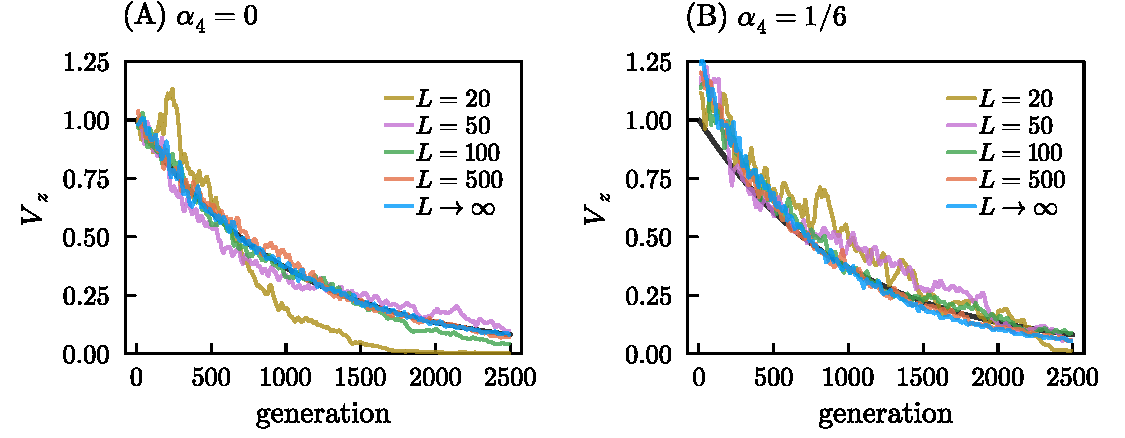
\includegraphics[width=0.8\linewidth]{/home/arzwa/dev/InfGenetics/doc/img/tetfininf.pdf}
%DIFDELCMD < %%%
\DIFdelendFL \DIFaddbeginFL 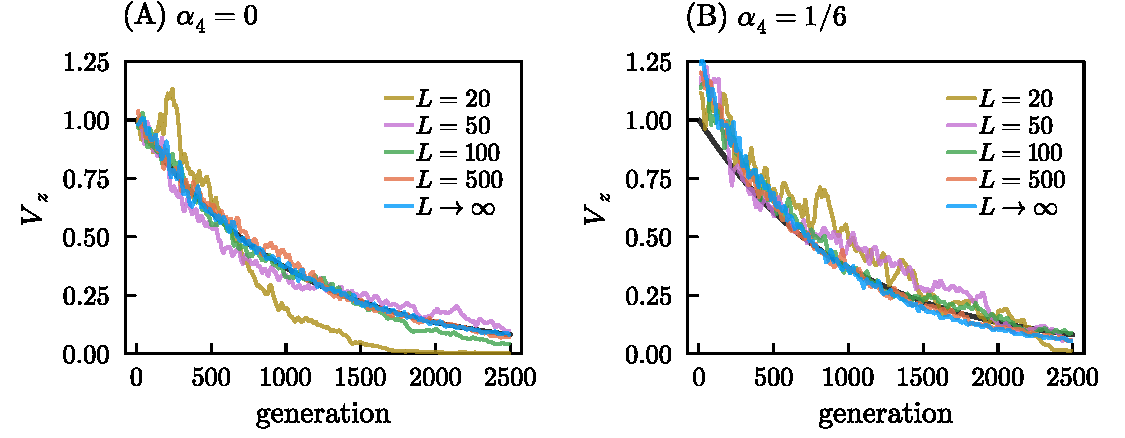
\includegraphics[width=0.8\linewidth]{/home/arzwa/dev/InfGenetics/doc/img/fig1.pdf}
\DIFaddendFL \caption{
The infinitesimal model in autotetraploids.
Comparisons are shown for the decay of the genetic variance ($V_z$) due to
inbreeding in exact simulations of the infinitesimal model in autotetraploids
against individual-based simulations of autotetraploid populations with $L$\DIFaddbeginFL \DIFaddFL{.
}\DIFaddendFL unlinked additive loci determining the quantitative trait. 
(A) Simulations of a model without double reduction ($\alpha_4=0$).
(B) Simulations of a model with maximal double reduction ($\alpha_4=1/6$) (for
all loci in the finite $L$ simulations).
We show window-smoothed values for visual clarity, with observed genetic
variances averaged in windows of 20 generations every 10 generations.
The black line marks $e^{-t/4N}$. 
We assume $N=250$ and $V_z(0) = 1$.
\label{fig:vztet}}
\end{figure}

We evaluate the accuracy of the autotetraploid infinitesimal model as an
approximation to the evolution of a quantitative trait determined by $L$
additive loci.
We find that the infinitesimal model with inbreeding generally yields accurate
predictions for the evolution of the genetic variance when the number of loci
is sufficiently large ($L \ge 100$, say, \cref{fig:vztet,s-fig:fininf}).
Furthermore, we confirm that, in the absence of double reduction, the decay in
genetic variance due to inbreeding after a time $t$ is well-predicted by
$e^{-t/4N}$ (\cref{fig:vztet}A), as expected from the results of \cite{arnold2012}.
As predicted, double reduction (i.e. $\alpha_4 > 0$) leads to an immediate
increase in genetic variance (as it increases the segregation variance), but
leads to accelerated inbreeding, causing faster loss of \DIFdelbegin \DIFdel{genetic variance }\DIFdelend \DIFaddbegin \DIFadd{variation }\DIFaddend in the
long term (\cref{fig:vztet,s-fig:fininf}).
Simulations for the mixed-ploidy model further confirm the correctness of our
infinitesimal approximation (\cref{s-fig:vz}).

It is worth noting that, although inbreeding is slower in autotetraploids than
in diploids for the same population size, the tetraploid fraction of a
diploid-dominated mixed-ploidy population will have an equal or higher average
inbreeding coefficient (\cref{s-fig:f1}).
This is because in such a population, triploid and tetraploid individuals
mostly arise from gametes formed by diploid individuals, or by polyploid
individuals with very recent diploid ancestry (on average $1+u+2v$ generations ago
for tetraploids, and $1+\frac{2}{3}(u+2v)$ generations ago for triploids, see
\cref{s-sec:ttdip}).
A nonzero probability of producing IBD diploid gametes ($\alpha_k > 0$) will
then further increase the inbreeding coefficient in the tetraploid and triploid
fraction of the population relative to their diploid progenitors
(\cref{s-fig:f1}).
Therefore, as long as diploids dominate, harboring some fraction of the gene
pool in polyploid individuals has a negligible effect on the rate of inbreeding
in the mixed-ploidy population as a whole, and we find that the evolution of
the inbreeding coefficient over time is well predicted by $1-e^{-t/2N_e}$,
where the inbreeding-effective population size is, to first order in $u$, given
by $(1-2u)N$ (\cref{s-sec:effsize}). This is just the expected number of
diploid individuals (to first order in $u$), highlighting that when diploids
dominate, polyploids \DIFdelbegin \DIFdel{have low fitness and }\DIFdelend do not contribute to the effective population size. 


\subsection*{Establishment from a single individual}

\begin{figure}[t]
\centering
\DIFdelbeginFL %DIFDELCMD < 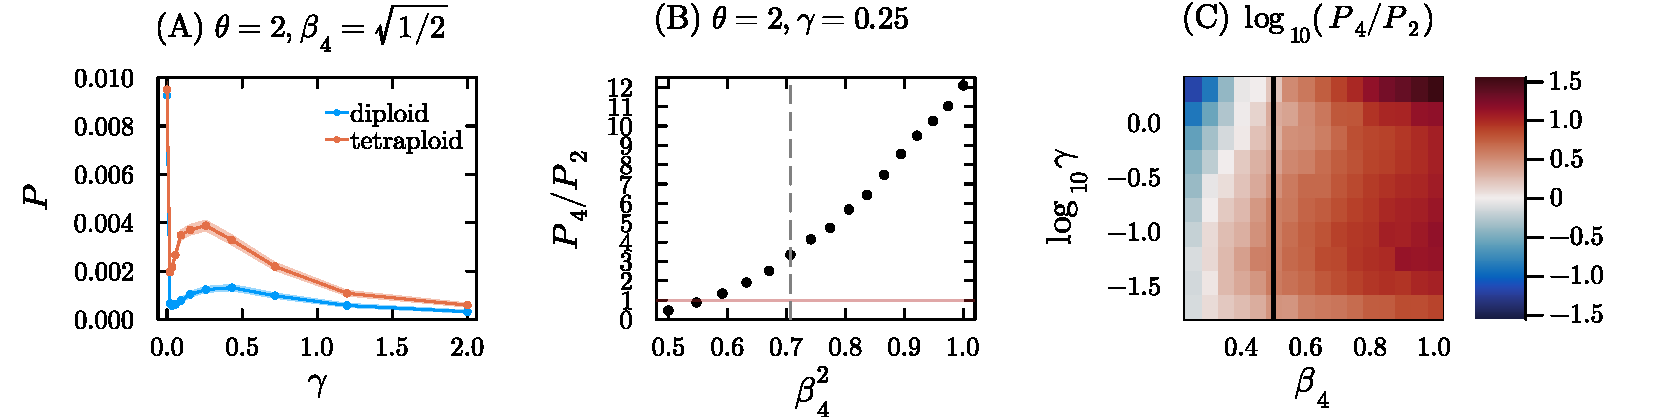
\includegraphics[width=\linewidth]{/home/arzwa/dev/InfGenetics/doc/img/est1b.pdf}
%DIFDELCMD < %%%
\DIFdelendFL \DIFaddbeginFL 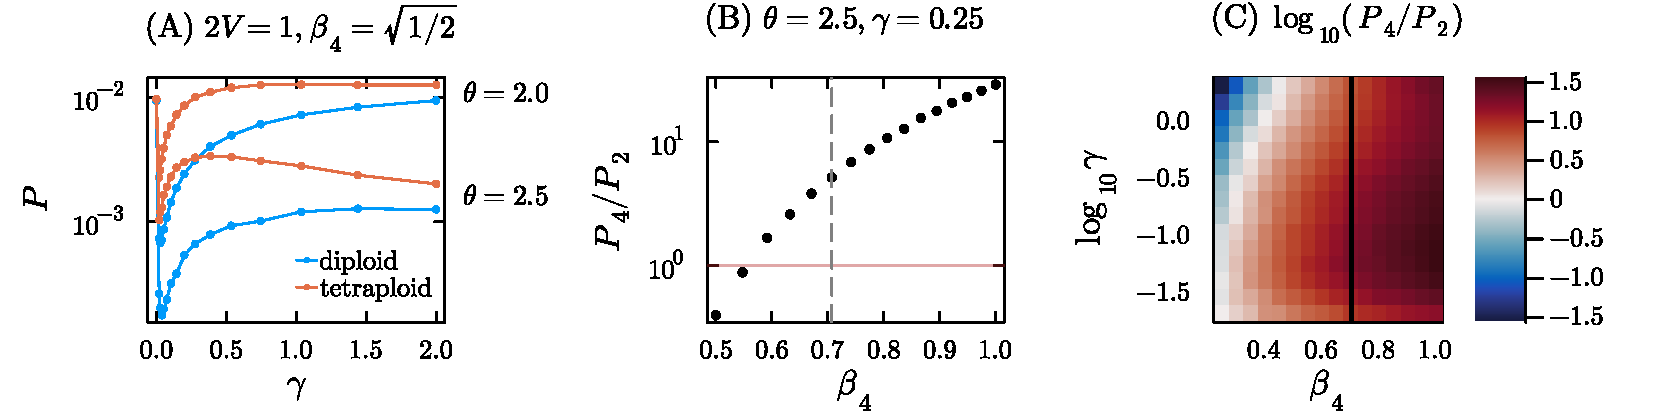
\includegraphics[width=\linewidth]{/home/arzwa/dev/InfGenetics/doc/img/fig2.pdf}
\DIFaddendFL \caption{
    (A) Probability of establishment \DIFaddbeginFL \DIFaddFL{(defined as reaching $N=100$) }\DIFaddendFL from a
    single diploid or tetraploid individual with trait value $z=0$ for
    increasing selection intensity $\gamma$\DIFaddbeginFL \DIFaddFL{, for two different values of
    $\theta$ (degree of maladaptation)}\DIFaddendFL .  We assume $m=0$ and $u=0$, i.e. there
    is no migration, and no unreduced gametes are produced. The trait is scaled
    in tetraploids so as to yield the same genetic variance at HWLE (\DIFdelbeginFL \DIFdelFL{$\beta_4 = \sqrt{1/2}$}\DIFdelendFL \DIFaddbeginFL \DIFaddFL{$\beta_4^2 =
    1/2$}\DIFaddendFL )\DIFaddbeginFL \DIFaddFL{.
    Note that when $\gamma = 0$, we obtain a critical branching process with a
    Poisson offspring distribution, so that the probability to reach $N=100$ is
    $\sim 1/100$ \mbox{%DIFAUXCMD
\citep{barton2018}}\hspace{0pt}%DIFAUXCMD
.  
}\DIFaddendFL (B) Probability of a tetraploid individual with trait value $z = 0$
    successfully founding a population ($P_4$), relative to the probability for
    a diploid individual with the same trait value ($P_2$).  The vertical
    dashed line marks \DIFdelbeginFL \DIFdelFL{$\beta_4=\sqrt{1/2}$, for which the variance at
HWLE is identical between diploids and autotetraploids}\DIFdelendFL \DIFaddbeginFL \DIFaddFL{$\beta_4^2=1/2$}\DIFaddendFL .
(C) Probability of tetraploid establishment relative to the probability of
    diploid establishment (on a $\log_{10}$ scale) across a range of values for
    $\gamma$ and $\beta_4$ \DIFaddbeginFL \DIFaddFL{($\theta=2.5$)}\DIFaddendFL . The vertical line again marks
    \DIFdelbeginFL \DIFdelFL{$\beta_4=\sqrt{1/2}$}\DIFdelendFL \DIFaddbeginFL \DIFaddFL{$\beta_4^2=1/2$}\DIFaddendFL .  All results are estimated from \DIFaddbeginFL \DIFaddFL{1.000.000 (A\&B) or
    }\DIFaddendFL 500.000 \DIFaddbeginFL \DIFaddFL{(C) }\DIFaddendFL replicate simulations\DIFdelbeginFL \DIFdelFL{and assume
$\theta=2$. Establishment is defined as reaching $N=100$}\DIFdelendFL .
\label{fig:est1}}
\end{figure}


Having established the validity of the mixed-ploidy infinitesimal model, we now
use it to study the establishment of polyploids in a marginal habitat to which
migrants from a mixed-ploidy source population are maladapted.

We first consider the establishment of a population from a single migrant
individual with trait value $z_0 = 0$.
We assume $u=0$ (i.e. there are no unreduced gametes, and hence no newly formed
polyploids) and compare the probability of establishment when the migrant
is diploid vs. tetraploid (\cref{fig:est1}).
\DIFdelbegin \DIFdel{As noted by \mbox{%DIFAUXCMD
\cite{barton2018}}\hspace{0pt}%DIFAUXCMD
}\DIFdelend \DIFaddbegin \DIFadd{For a given mixed-ploidy model (characterized by parameters $\alpha, \beta,
u$ and $v$)}\DIFaddend , the establishment probability \DIFdelbegin \DIFdel{(for a given
cytotype) depends essentially on }\DIFdelend \DIFaddbegin \DIFadd{depends on $\gamma, \theta$ and $V$
through }\DIFaddend two dimensionless parameters, $\gamma\sqrt{2V}$ and $\theta/\sqrt{2V}$
\DIFaddbegin \DIFadd{\mbox{%DIFAUXCMD
\citep{barton2018}}\hspace{0pt}%DIFAUXCMD
}\DIFaddend , corresponding to the intensity of selection and the degree
of maladaptation, respectively.
We shall scale our results accordingly, assuming $2V=1$ throughout\DIFdelbegin \DIFdel{, and shall
assume $\theta=2$, so that the average trait value has to increase by two
standard deviations to achieve a positive growth rate.
The }\textit{\DIFdel{relative}} %DIFAUXCMD
\DIFdel{establishment probability for different cytotypes will of
course also depend on how allelic effects scale across ploidy levels ($\beta_4$)}\DIFdelend .

\DIFdelbegin \DIFdel{We }\DIFdelend \DIFaddbegin \DIFadd{For a fixed degree of maladaptation $\theta$, the probability of establishment
depends in a complicated way on the strength of selection.
To see this, note that the expected number of offspring of an initial migrant
of ploidy level $k$ is $e^{-\gamma \theta + \gamma^2 k\beta_k^2 V/4}$, and the
expected trait value among its offspring will be $\gamma k \beta_k^2 V/2$.
A higher intensity of selection ($\gamma$) therefore yields a stronger effect
of initial maladaptation, but also causes a stronger response in the mean trait
value.
If the genetic variance is not constant across cytotypes (i.e. $\beta_4^2 \ne
1/2$), this response will differ for different ploidy levels.
Different rates of inbreeding due to differences in ploidy level will then
further cause rates of adaptation to differ, leading to different establishment
probabilities, even when $\beta_4^2=1/2$.
}

\DIFadd{Indeed, we }\DIFaddend find that reduced inbreeding in tetraploids substantially increases the
\DIFdelbegin \DIFdel{establishment probability of tetraploids }\DIFdelend \DIFaddbegin \DIFadd{likelihood of tetraploid establishment }\DIFaddend relative to diploids across a large
part of the parameter space (\cref{fig:est1}\DIFdelbegin \DIFdel{).
Indeed, in the case where allelic effects are scaled across ploidy levels
to yield the same equilibrium genetic variance ($\beta_4 = \sqrt{1/2}$, so that
polyploid migrants are not more likely to have high fitness than diploid
migrants)}\DIFdelend \DIFaddbegin \DIFadd{A).
For the $\beta_4^2 = 1/2$ case}\DIFaddend , the establishment probability for
tetraploids can be \DIFdelbegin \DIFdel{almost five
}\DIFdelend \DIFaddbegin \DIFadd{more than ten }\DIFaddend times as high as \DIFdelbegin \DIFdel{in }\DIFdelend \DIFaddbegin \DIFadd{for }\DIFaddend diploids depending on the
selection gradient (\DIFaddbegin \DIFadd{$\gamma$) and the degree of maladaptation ($\theta$)
(}\DIFaddend \cref{fig:est1}A).
As the segregation variance and initial trait value are the same across these
simulations, this is a consequence only of the reduced rate of inbreeding,
which slows down the exhaustion of the genetic variance carried by the initial
migrant individual.
\DIFdelbegin %DIFDELCMD < 

%DIFDELCMD < %%%
\DIFdel{While the probability of establishment becomes lower as the strength of
selection becomes large, the establishment probability does not decrease
monotonically with $\gamma$, i.e. as selection becomes very weak, the
establishment probability also decreases.
This happens because, although the probability of surviving the first couple of
generations becomes higher when selection is weaker, adaptation (i.e. increase
in the trait mean) will be slower,
increasing the risk that genetic variation is exhausted due to inbreeding before the
population is able to reach a consistently positive growth rate.
Note that when $\gamma = 0$, each individual has fitness 1 and we have a
critical branching process with a Poisson offspring distribution, so that the
probability to reach $N=100$ is $1/100$ \mbox{%DIFAUXCMD
\citep{barton2018}}\hspace{0pt}%DIFAUXCMD
.  
}%DIFDELCMD < 

%DIFDELCMD < %%%
\DIFdelend Evidently, the scaling of the genetic variance across ploidy levels has a
profound effect on the establishment probability, but only when $\beta_4$ is
close to 0.5 (i.e. individual alleles have almost half the effect size in
tetraploids compared to diploids) is the benefit of the slower rate of
inbreeding in tetraploids canceled \DIFaddbegin \DIFadd{by the reduction in the equilibrium genetic
variance }\DIFaddend (\cref{fig:est1}B,C).



\subsection*{Establishment with recurrent migration}

\begin{figure}[t]
\centering
\DIFdelbeginFL %DIFDELCMD < 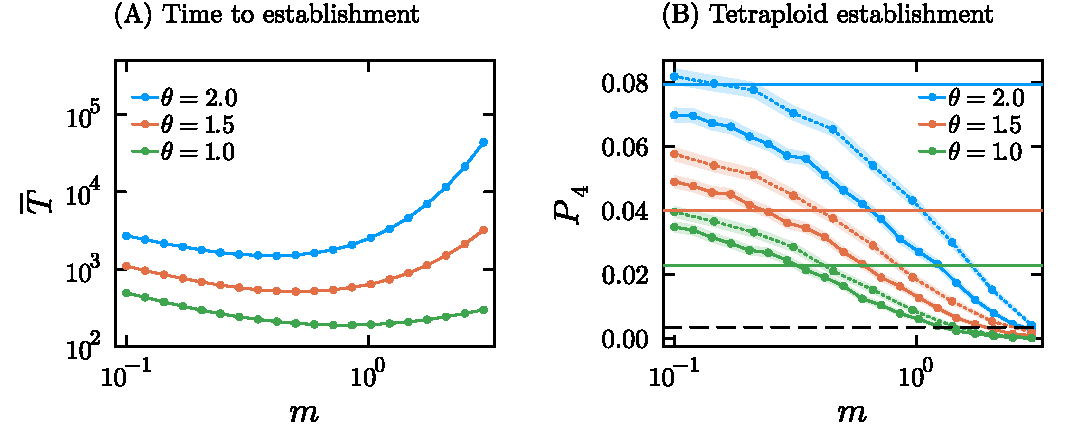
\includegraphics[width=0.8\linewidth]{/home/arzwa/dev/InfGenetics/doc/img/estwmigration-dr.pdf}
%DIFDELCMD < %%%
\DIFdelendFL \DIFaddbeginFL 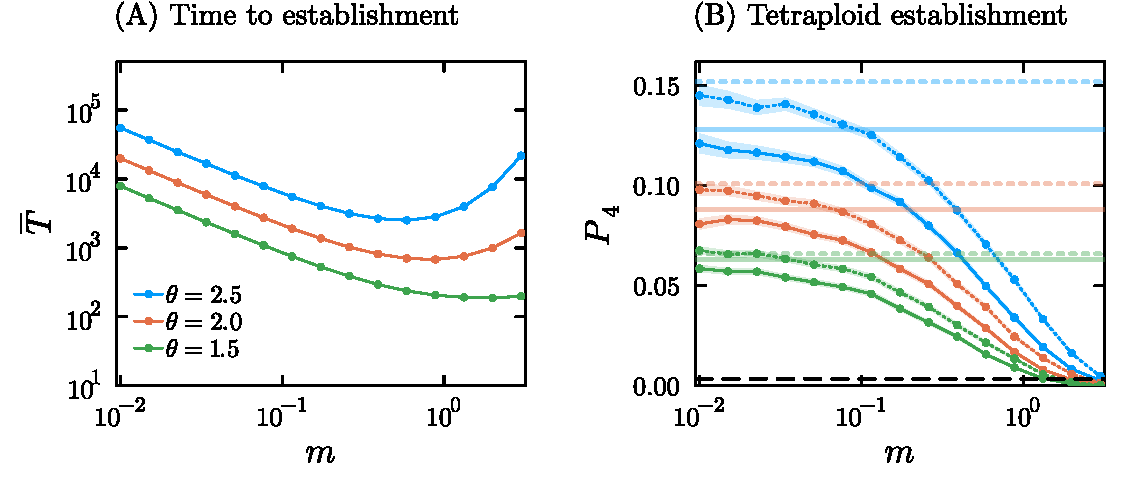
\includegraphics[width=0.8\linewidth]{/home/arzwa/dev/InfGenetics/doc/img/fig3.pdf}
\DIFaddendFL \caption{
    Establishment with recurrent migration.
    (A) Expected time until a population is established in the marginal habitat
    for increasing rates of migration and different degrees of maladaptation
    ($\theta$). Results are shown for the case with $\alpha_k = 0$ for
    $k=2,3,4$. 
    (B) Proportion of simulation replicates in which tetraploids established.
    The dots connected by solid lines show simulation results with
    $\alpha_k=0$, whereas the dots connected by dashed lines
    show simulation results with $\alpha_2=1/2, \alpha_3=1/4$ and
    $\alpha_4=1/6$ (i.e. maximum $\alpha$).
    The \DIFdelbeginFL \DIFdelFL{solid }\DIFdelendFL horizontal lines mark \DIFdelbeginFL \DIFdelFL{$\frac{p_4\pi_4}{(p_4\pi_4 + p_2\pi_2)}$,
    where $p_2$ and $p_4$ are }\DIFdelendFL the establishment probabilities \DIFdelbeginFL \DIFdelFL{for a single
    diploid and a single tetraploid individual }\DIFdelendFL in the
    \DIFdelbeginFL \DIFdelFL{absence of migration (}\DIFdelendFL \DIFaddbeginFL \DIFaddFL{limit }\DIFaddendFL as \DIFdelbeginFL \DIFdelFL{in }%DIFDELCMD < \cref{fig:est1}%%%
\DIFdelFL{, but with unreduced gamete formation included}\DIFdelendFL \DIFaddbeginFL \DIFaddFL{$m\rightarrow 0$ (solid lines: without double reduction; dashed
    lines: maximum $\alpha$}\DIFaddendFL ).
    The \DIFdelbeginFL \DIFdelFL{dashed }\DIFdelendFL \DIFaddbeginFL \DIFaddFL{black }\DIFaddendFL horizontal line marks the proportion of tetraploid migrants
    (i.e. the proportion of tetraploids at equilibrium in the source
    population, $\approx 0.3$\%).
    The baseline predictions (horizontal lines) are based on \DIFdelbeginFL \DIFdelFL{$5\times 10^6$
    }\DIFdelendFL \DIFaddbeginFL \DIFaddFL{500.000 }\DIFaddendFL simulation
    replicates.
    All other results are based on \DIFdelbeginFL \DIFdelFL{50.000 }\DIFdelendFL \DIFaddbeginFL \DIFaddFL{100.000 }\DIFaddendFL replicate simulations.
    We assume $\gamma=0.25$ and $u=v=0.05$.
    \label{fig:estwmig}}
\end{figure}

We next consider establishment in the new habitat when there is a continuous
influx of migrants ($m$ migrants per generation on average) coming from a large,
noninbred and predominantly diploid source population at cytotype equilibrium.
In this setting, establishment is certain to happen eventually, and we are
interested in the probability that a tetraploid population establishes before a
diploid one does.

We hypothesized that two counteracting processes affect the probability of
autotetraploid establishment in this scenario.
On the one hand, increased migration will increase the probability that an
otherwise likely successful tetraploid migrant suffers from MCE in the early
generations while the population size is low, because migrants are likely to be
diploid.
On the other hand, tetraploids are more strongly reproductively isolated from
a typical migrant, so that a tetraploid subpopulation should be less prone to
maladaptive gene flow.
Hence, conditional on evading MCE, they should be able to adapt to the new
habitat at a rate which is not strongly affected by the migration rate.
This contrasts with diploids, which interbreed freely with maladapted
migrants, resulting in a pulling back of the trait mean towards that of the
source population.
Lastly, as the mean trait value on the island increases in diploids
during adaptation, tetraploid offspring will have more extreme phenotypes on
average than diploid offspring when $\beta_4 > 1/2$, which may also aid their
establishment (irrespective of $m$).

\begin{figure}[t]
\centering
\DIFdelbeginFL %DIFDELCMD < 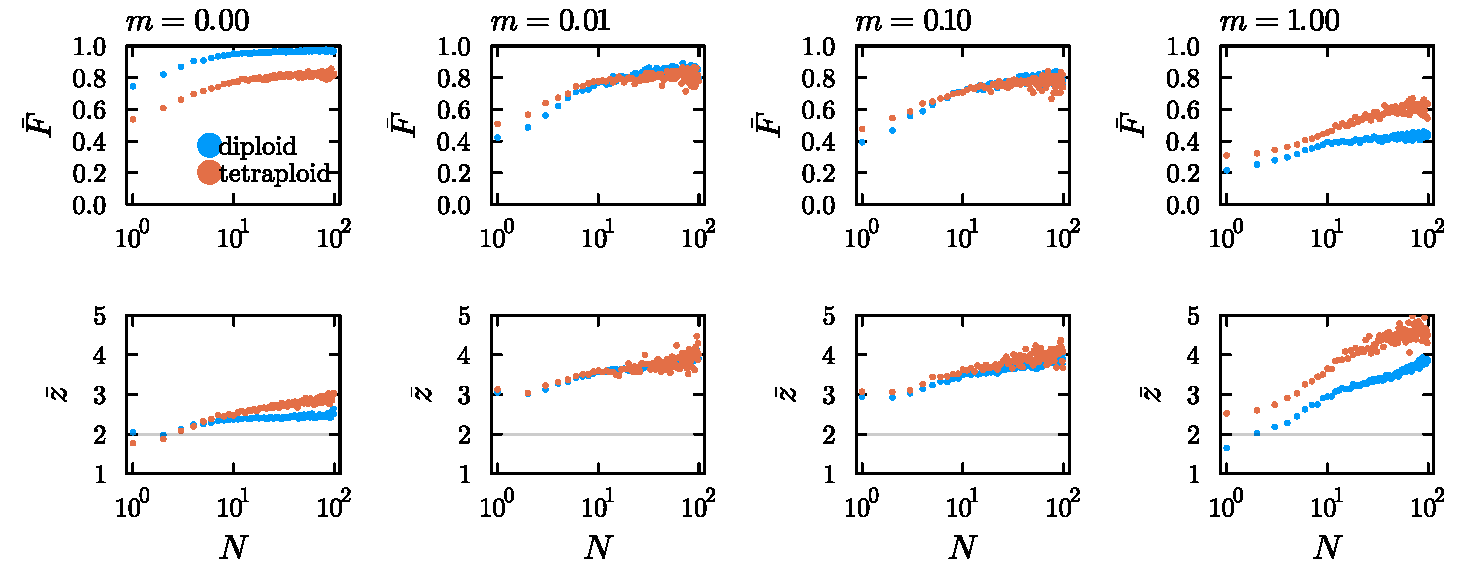
\includegraphics[width=\linewidth]{/home/arzwa/dev/InfGenetics/doc/img/estwmigration1d.pdf}
%DIFDELCMD < %%%
\DIFdelendFL \DIFaddbeginFL 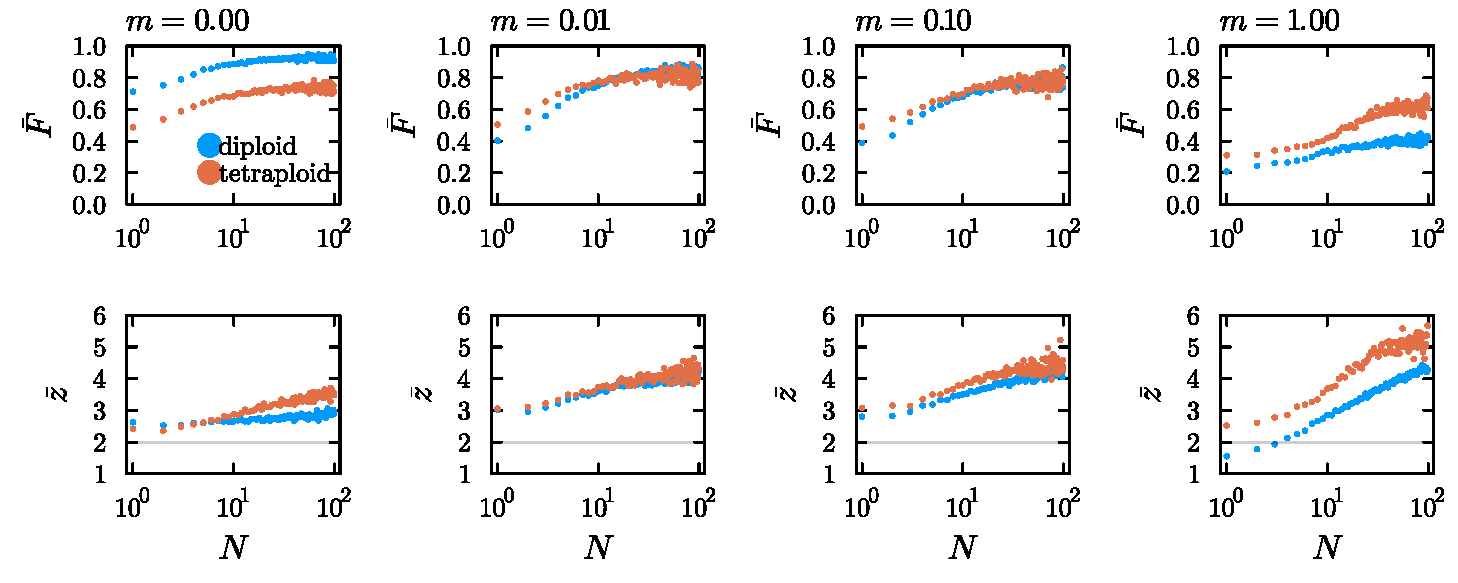
\includegraphics[width=\linewidth]{/home/arzwa/dev/InfGenetics/doc/img/fig4.pdf}
\DIFaddendFL \caption{
    Evolution of the mean inbreeding coefficient and trait value across
    simulation replicates where diploids (blue) or tetraploids (orange)
    established eventually.
    Average $F$ and $z$ by population size are shown for increasing rates
    of migration ($m$) from the predominantly diploid source population. 
    All results are based on 1000 succesful establishment replicates.
    We assume equal equilibrium variance across ploidy levels and $\gamma=0.25,
    \theta=2, 2V=1$ and $u=v=0.05$.
    \DIFdelbeginFL \DIFdelFL{The }\DIFdelendFL \DIFaddbeginFL \DIFaddFL{For the }\DIFaddendFL $m=0$ simulations\DIFdelbeginFL \DIFdelFL{are seeded with a single diploid or tetraploid
    individual with }\DIFdelendFL \DIFaddbeginFL \DIFaddFL{, the }\DIFaddendFL trait value \DIFdelbeginFL \DIFdelFL{0}\DIFdelendFL \DIFaddbeginFL \DIFaddFL{of the initial migrant was
    Gaussian with mean zero and variance $2V$}\DIFaddendFL , and \DIFdelbeginFL \DIFdelFL{assume }\DIFdelendFL $u=v=0$ \DIFaddbeginFL \DIFaddFL{is assumed}\DIFaddendFL .
\label{fig:estwmig2}}
\end{figure}

As expected, we find that the time to establishment (of a population of either
ploidy level) first decreases with increasing migration as a result of a larger
influx of potentially succesful migrants, but later increases with increasing
migration due to swamping by gene flow (\cref{fig:estwmig}A).
Importantly, the tetraploid establishment probability is considerably larger
than the expected proportion of tetraploid migrants over \DIFdelbegin \DIFdel{a large part of the parameter range }\DIFdelend \DIFaddbegin \DIFadd{almost the entire
parameter range examined }\DIFaddend (\cref{fig:estwmig}B, black dashed line).
\DIFdelbegin \DIFdel{Furthermore, we find that for small migration rates}\DIFdelend \DIFaddbegin \DIFadd{However}\DIFaddend , the probability \DIFdelbegin \DIFdel{that
tetraploids establish rather than diploids can be larger than expected based on
the establishment probabilities in the absence of migration (colored lines in
}%DIFDELCMD < \cref{fig:estwmig}%%%
\DIFdel{), depending on how maladapted migrant individuals are.
This suggests that maladaptive gene flow in diploids can increase the
probability of tetraploid establishment.
However, at the same time we find that the tetraploid establishment probability
declines monotonically
with $m$, which highlights }\DIFdelend \DIFaddbegin \DIFadd{of tetraploid establishment does decline monotonically
with the migration rate, showing that }\DIFaddend the negative effects of MCE \DIFdelbegin \DIFdel{.
Together, these results confirm the view that, while cytotype differences are an
effective barrier to }\DIFdelend \DIFaddbegin \DIFadd{on tetraploid
establishment outweigh the positive effects of reduced }\DIFaddend maladaptive gene flow \DIFdelbegin \DIFdel{, this advantage to establishment is
outweighed by the negative effects of MCE}\DIFdelend \DIFaddbegin \DIFadd{in
the absence of prezygotic isolation}\DIFaddend .

Our simulations further show that the mechanism of unreduced gamete formation
(as determined by the $\alpha_2$ parameter) can affect the establishment
probability (\cref{fig:estwmig}B, dashed lines).
This is mainly because the phenotypic variance of a newly formed tetraploid is
increased by a factor $(1+\alpha_2)$, thereby increasing the chance that a
tetraploid migrant is well-adapted to the marginal habitat.
The rate of double reduction ($\alpha_4$) has a more limited effect
(\cref{s-fig:suppdr}).

Established diploid populations are more inbred on average than established
tetraploids when migration is weak, but the difference is slight except when
there is no migration at all (\cref{fig:estwmig2}, top row).
For stronger migration ($m > 0.1$), the opposite holds.
This is a result of two interacting processes.
On the one hand, inbreeding is slower in tetraploids, so that during adaptation
and establishment from a single or limited number of outbred individuals, 
the inbreeding coefficient is expected to increase less rapidly\DIFdelbegin \DIFdel{conditional on
the event of tetraploid establishment}\DIFdelend .
On the other hand, migration mostly introduces unrelated diploids, which cross
more readily with diploids than tetraploids, reducing the average relatedness
more strongly in established diploid than in tetraploid populations.

Conditional on establishment, tetraploids have a higher trait mean \DIFdelbegin \DIFdel{both in the
absence of migration and for moderate to strong migration, but not when
migration is weak }\DIFdelend \DIFaddbegin \DIFadd{than
diploids }\DIFaddend (\cref{fig:estwmig2}, bottom row).
In the absence of migration, this is a consequence of the reduced rate of
inbreeding and the resulting increased adaptive potential of tetraploids.
\DIFdelbegin \DIFdel{Another consequence of this is that the average trait value in tetraploids at
low population size (}\DIFdelend \DIFaddbegin \DIFadd{For weak migration, the difference in trait values between diploids and
tetraploids, }\DIFaddend conditional on eventual establishment\DIFdelbegin \DIFdel{) is lower than that
in diploids.
This is because, in
order to adapt before genetic variation is exhausted,
tetraploids need not increase the trait mean as much as diploids do in the first couple of generations.
The similar trait means for weak migration suggest that establishment depends
mostly on the chance pick of a well-adapted migrant (note that the $m=0$
simulations in
}%DIFDELCMD < \cref{fig:estwmig2} %%%
\DIFdel{assume the initial migrant has $z=0$,
whereas the $m=0.01$ simulations assume the initial trait value to be
Gaussian)}\DIFdelend \DIFaddbegin \DIFadd{, is limited.
This indicates the beneficial effects of migration on establishment in
diploids: migration introduces new variation on which selection can act,
counteracting the loss of genetic variance due to inbreeding.
The genetic variance contributed by migration is however negligible in
tetraploids}\DIFaddend .
When migration is strong, tetraploids have markedly larger trait values
than diploids ($m=1$ in \cref{fig:estwmig2}), showing that diploids suffer
strongly from maladaptive gene flow when the population size is low, while
tetraploids \DIFdelbegin \DIFdel{enjoy some reproductive isolation}\DIFdelend \DIFaddbegin \DIFadd{are much more reproductively isolated from migrants}\DIFaddend .
Furthermore, in these replicates, tetraploids tend to emerge and rise in
frequency at larger population sizes on the island, and hence tend to derive
from diploids that already experienced several generations of selection.
These neotetraploids, deriving from diploid parents with $z>0$, will have more
extreme phenotypes on average (see methods) and hence be better adapted.


\subsection*{Loss of self-incompatibility, selfing and assortative mating}

When polyploidization disrupts an existing SI system (see e.g.
\cite{robertson2011comparative,zenil2019,novikova2023}), we expect that
tetraploids suffer less from MCE, as some portion of their ovules are now
assured to be fertilized by diploid gametes, irrespective of the composition of
the population.
At the same time, we expect that accelerated inbreeding in selfing tetraploids
diminishes the adaptive advantage of tetraploids.
We find that when polyploidization is associated with the loss of a SI system
(i.e. when diploids are self-incompatible, but tetraploids are not),
tetraploids have a strongly increased establishment probability
(\cref{fig:selfing}).
This is the case even when the selfing rate $\sigma$ in tetraploids is zero (in
which case, under our modeling assumptions, there is only random selfing, i.e.
the \textit{realized} selfing rate in tetraploids is $1/N$).
Furthermore, we find that when the selfing rate is sufficiently high ($\ge 0.4$
in \cref{fig:selfing}A), the relative establishment probability of tetraploids
increases with increasing migration rate.
In this regime, the \DIFdelbegin \DIFdel{increased strength of MCE due to increased migration and
increased }\DIFdelend \DIFaddbegin \DIFadd{effects of migration on MCE and }\DIFaddend reproductive assurance in
diploids \DIFdelbegin \DIFdel{is }\DIFdelend \DIFaddbegin \DIFadd{are }\DIFaddend compensated by the stronger maladaptive gene flow experienced by
diploids.

Self-incompatibility is clearly a strong disadvantage when colonizing a novel
habitat, as a self-incompatible population of size one can never reproduce.
However, even when diploids are self-compatible, polyploids may still have
increased rates of self-fertilization (for instance due to altered flower
morphology).
For the sake of comparison, \cref{fig:selfing}A also shows results where
diploids are assumed to be self-compatible with $\sigma_2=0$ (i.e. random
selfing, dashed transparent lines).
The tetraploid establishment probability is still markedly increased when
$\sigma_4 \ge 0.4$, and as for the simulations with self-incompatibility,
migration still promotes the probability of tetraploid establishment when the
selfing rate in polyploids is sufficiently large compared to the diploid
selfing rate.

\begin{figure}
\centering
\DIFdelbeginFL %DIFDELCMD < 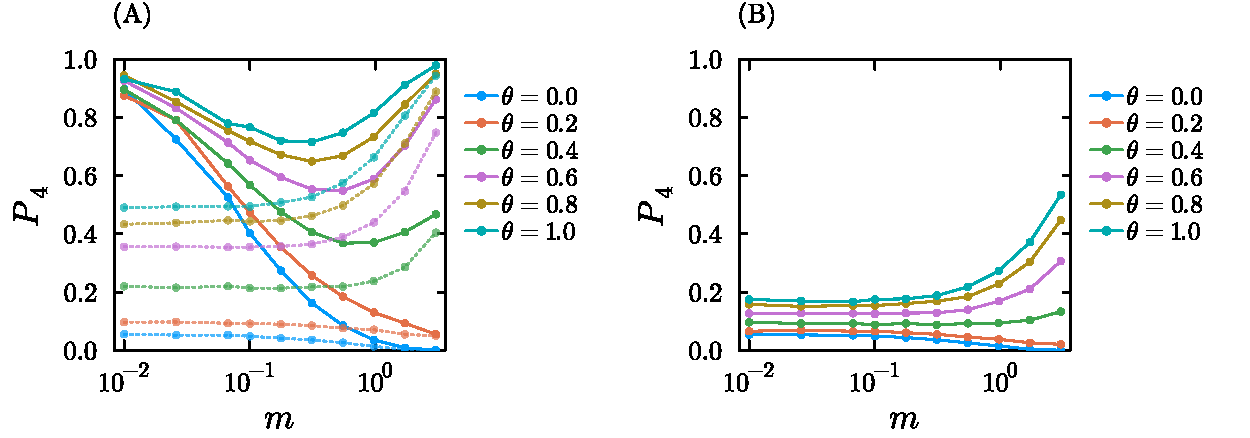
\includegraphics[width=0.9\linewidth]{/home/arzwa/dev/InfGenetics/doc/img/prez.pdf} 
%DIFDELCMD <     %%%
\DIFdelendFL \DIFaddbeginFL 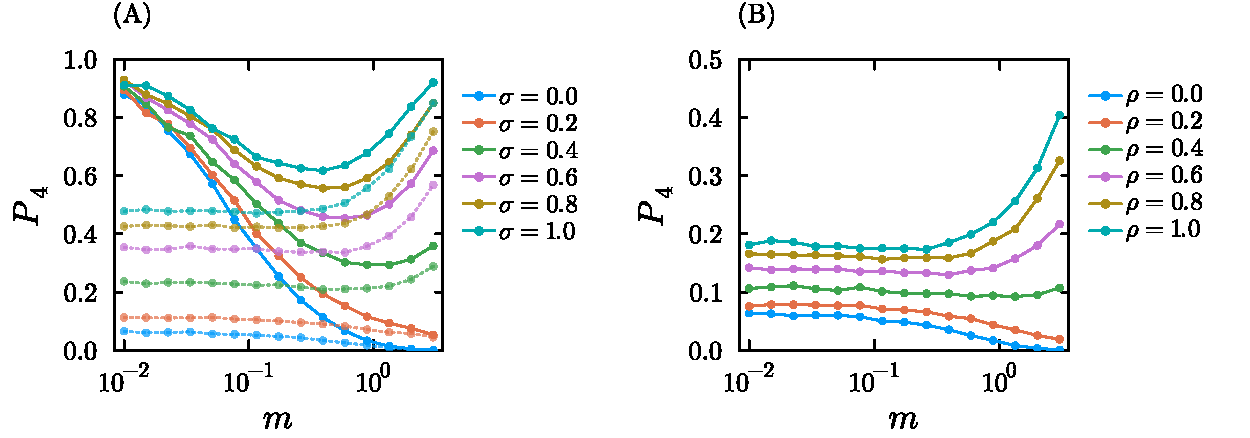
\includegraphics[width=0.9\linewidth]{/home/arzwa/dev/InfGenetics/doc/img/fig5.pdf} 
    \DIFaddendFL \caption{
    (A) Establishment with recurrent migration \DIFaddbeginFL \DIFaddFL{and }\DIFaddendFL selfing in polyploids. 
    The solid lines show the case where diploids are self-incompatible 
    The dashed transparent lines show the case where diploids do random
    self-fertilization (i.e. self-fertilization occurs with probability $1/N$),
    Triploids and tetraploids have the same selfing rate. 
    $\sigma=0.0$ refers to random self-fertilization.  
    (B) Establishment with recurrent migration and assortative mating by
    cytotype. The rate of assortative mating is determined by $\rho_k = \rho$
    for $k=2,3,4$, where $\rho_k$ is the probability that an ovule from a
    $k$-ploid mother is pollinated by a $k$-ploid father.
    All results are based on \DIFdelbeginFL \DIFdelFL{25.000 }\DIFdelendFL \DIFaddbeginFL \DIFaddFL{50.000 }\DIFaddendFL replicate simulations.  We assume
    \DIFdelbeginFL \DIFdelFL{$\gamma=0.25, \theta=1.5$ }\DIFdelendFL \DIFaddbeginFL \DIFaddFL{$\gamma=0.25, \theta=2$ }\DIFaddendFL and $u=v=0.05$.  \label{fig:selfing}}
\end{figure}

Another prezygotic isolating mechanism that has often been considered relevant
for explaining tetraploid establishment is assortative mating by ploidy level,
where ovules from a tetraploid are more likely to be fertilized by
pollen coming from a tetraploid -- irrespective of the trait values of these
individuals.
Clearly, assortative mating increases the probability of tetraploid
establishment (\cref{fig:selfing}B), although not as strongly as the loss of an SI
system does.
Again, we find that for some parameter values (roughly $\rho \ge 0.4$),
assortative mating may be strong enough so that tetraploid establishment
increases with increasing migration rates, suggesting that tetraploids evade
maladapive gene flow sufficiently to overcome MCE.
Note that the case $\rho = 1$ amounts to complete prezygotic isolation.

\section*{Discussion}

The observation that polyploid populations tend to inhabit more extreme
habitats or occur at the edge of the range of their conspecific diploids
has spurred considerable interest among botanists and evolutionary biologists
\DIFdelbegin \DIFdel{\mbox{%DIFAUXCMD
\citep{rice2015,kolar2017,vandepeer2021,griswold2021,mortier2024}}\hspace{0pt}%DIFAUXCMD
}\DIFdelend \DIFaddbegin \DIFadd{\mbox{%DIFAUXCMD
\citep{kolar2017,rice2019,vandepeer2021,griswold2021,mortier2024}}\hspace{0pt}%DIFAUXCMD
}\DIFaddend .
An important question is whether such patterns emerge because polyploids are
somehow more tolerant to extreme environmental conditions (i.e. they somehow
are intrinsically more fit than diploids in marginal habitats), or whether other
aspects of the population dynamics of mixed-ploidy populations may favor the
establishment of polyploid subpopulations.

In this study, we worked out the infinitesimal model for an additive polygenic
trait in autotetraploids and mixed-ploidy populations and used it to study the
establishment of tetraploids in a marginal habitat by means of individual-based
simulations.
Assuming the trait to be under directional selection in the marginal habitat,
and migration of maladapted individuals from a predominantly diploid source,
we sought to determine \DIFdelbegin \DIFdel{the conditions under which }\DIFdelend \DIFaddbegin \DIFadd{under which conditions }\DIFaddend tetraploids are more likely to
establish a stable population.

\DIFaddbegin \DIFadd{Throughout, we have assumed a relatively high and constant rate of unreduced
gamete formation $u$ and triploid fertility $v$ in all our simulations (5\%),
whereas these are known to be variable across the population, and at least in
part genetically determined \mbox{%DIFAUXCMD
\citep{kreiner2017,clo2022c}}\hspace{0pt}%DIFAUXCMD
.
We ignore such complications, and hence do not take the actual establishment
probabilities very serious, focusing instead on how migration load and
prezygotic isolation affect the tetraploid establishment probability.
}

\DIFadd{Similarly, we have ignored mutation, which would reduce the rate at which
genetic variation is lost through inbreeding \mbox{%DIFAUXCMD
\citep{barton2017}}\hspace{0pt}%DIFAUXCMD
, and would
likely do so differently across cytotypes (i.e. $\mu V_m$ is expected to differ
for different ploidy levels, where $\mu$ is the mutation rate and $V_m$ the
mutational variance).
The contribution of new mutation to the genetic variance on the timescales we
consider should however be very limited.
Indeed, any individual at the time of establishment derives from a completely
outbred migrant individual a relatively short time in the past, so that the
opportunity for mutation to contribute to differences in establishment
probability between diploids and tetraploids is negligible for realistic
$\mu V_m$.
}

\DIFaddend Importantly, we \DIFdelbegin \DIFdel{assume }\DIFdelend \DIFaddbegin \DIFadd{assumed }\DIFaddend no intrinsic advantage or disadvantage of polyploids in
the marginal habitat, i.e. the expected fitness of a migrant individual is the
same regardless of the ploidy level.
Differences in \DIFdelbegin \DIFdel{establishment probabilities }\DIFdelend \DIFaddbegin \DIFadd{the likelihood of polyploid establishment }\DIFaddend are hence caused
solely by aspects of autopolyploid genetics and the barrier to gene flow
between subpopulations of different ploidy levels.
This is undoubtedly unrealistic\DIFaddbegin \DIFadd{, as both trait values and fitness will often
differ systematically across ploidy levels (see e.g. \mbox{%DIFAUXCMD
\cite{porturas2019}}\hspace{0pt}%DIFAUXCMD
)}\DIFaddend .
For instance, neopolyploids are likely to suffer intrinsic fertility issues due
to meiotic irregularities associated with multivalent formation
\citep{bomblies2016,novikova2023}\DIFdelbegin \DIFdel{.
Furthermore, in our simulations, we have focused on the case where the }\DIFdelend \DIFaddbegin \DIFadd{, and triploids may be inviable due to
issues with endosperm development \mbox{%DIFAUXCMD
\citep{bretagnolle1995}}\hspace{0pt}%DIFAUXCMD
.
}

\DIFadd{Similarly implausible is the assumption of a constant }\DIFaddend equilibrium genetic
variance \DIFdelbegin \DIFdel{is constant }\DIFdelend across cytotypes (\DIFdelbegin \DIFdel{$\beta_4=\sqrt{1/2}$
}\DIFdelend \DIFaddbegin \DIFadd{$\beta_4^2=1/2$ }\DIFaddend in our model)\DIFdelbegin \DIFdel{.
It would be very interesting to experimentally assess whether typical
quantitative traits in mixed-ploidy populations follow approximately the
mixed-ploidy infinitesimal model we outlined in
this paper, and to actually
estimate how the }\DIFdelend \DIFaddbegin \DIFadd{, which we used in
most of our results (but see }\cref{fig:est1}\DIFadd{).
Empirical data on how the genetic }\DIFaddend variance scales across ploidy levels \DIFdelbegin \DIFdel{.
In addition, we have assumed a relatively high and constant rate of
unreduced
gamete formation $u$ and triploid fertility $v$ in all our simulations (5\%) ,
whereas these are known to be variable across the population, and at least in part genetically determined \mbox{%DIFAUXCMD
\citep{kreiner2017,clo2022c}}\hspace{0pt}%DIFAUXCMD
.
We ignore such complications, and hence do not take the actual establishment 
probabilities very serious, focusing instead on how migration load and prezygotic isolation affect the tetraploid establishment probability}\DIFdelend \DIFaddbegin \DIFadd{is scant
and suggests that there is no general rule \mbox{%DIFAUXCMD
\citep{gallais2003,porturas2019}}\hspace{0pt}%DIFAUXCMD
.
The meta-analysis performed by \mbox{%DIFAUXCMD
\cite{porturas2019} }\hspace{0pt}%DIFAUXCMD
does indicate that trait
variance across ploidy levels is often fairly constant, so the assumption of
equal genetic variance is arguably a reasonable default.
It should be noted however that other authors have made different assumptions
on how allelic effects (and hence genetic variance) scale across ploidy levels
(in particular \mbox{%DIFAUXCMD
\cite{griswold2021}}\hspace{0pt}%DIFAUXCMD
, who scaled allelic effects in a way that is
equivalent to $\beta_4 = 1/2$ in our model).
Such assumptions evidently impact the likelihood of polyploid establishment 
(}\cref{fig:est1}\DIFadd{).
More empirical data on quantitative traits in experimental or natural
mixed-ploidy populations is needed to assess whether the mixed-ploidy
infinitesimal model can adequately describe the genetics of quantitative traits
across cytotypes, and to suggest plausible values for the relevant parameters
($\alpha, \beta$)}\DIFaddend .

When migration is weak, succesful establishment is not affected by
maladaptive gene flow and we can treat establishment in the marginal habitat as
independent trials of founding a population from a single individual.
In order to avoid extinction, the population has to increase the trait mean
by a sufficient amount before the genetic variation carried by the initial
migrant individual is exhausted.
The probability that the population manages to do so depends on the degree of
maladaptation, the intensity of selection and the rate of inbreeding.
We find that the decreased rate of inbreeding in autotetraploids gives a
rare tetraploid migrant a larger adaptive potential than a diploid migrant,
even if the genetic variance carried by the founding individual is the same.

In the presence of maladaptive gene flow, a nascent tetraploid subpopulation
suffers from MCE, and although polyploids are more reproductively isolated from
a typical migrant (and hence suffer less maladaptive gene flow), MCE will
increasingly hamper the establishment of tetraploids as the rate of migration
grows.
Nevertheless, it is important to remark that despite MCE, the probability of
tetraploid establishment in the marginal habitat can be an order of magnitude
higher than expected based on the frequency of tetraploid migrants (i.e. is
roughly \DIFdelbegin \DIFdel{$O(u)$ instead of $O(u^2)$}\DIFdelend \DIFaddbegin \DIFadd{of order $u$ instead of $u^2$}\DIFaddend ) when migration is sufficiently weak and
maladaptation sufficiently high.

Additional sources of prezygotic isolation such as selfing and assortative
mating by cytotype may further boost the probability of tetraploid
establishment.
These processes interact with the rate of migration, so that when
selfing/assortative mating occurs above some threshold rate, the tetraploid
establishment probability increases with increasing migration rates, whereas
below the threshold it decreases with increasing migration pressure.
In the latter case, the advantage that tetraploids have when it comes to
avoiding maladaptive gene flow is not strong enough to overcome the effects of
MCE, whereas in the former case it is.

A major weakness of the present work, and an important caveat, is that we have
ignored inbreeding depression and dominance throughout.
Including dominance in the infinitesimal framework is already challenging for
diploids (requiring the tracking of four-way identity coefficients;
\cite{barton2023}), and appears intractable for higher ploidy levels.
However, autopolyploidy has important consequences whenever dominance is
relevant, as in the case of inbreeding depression
\DIFdelbegin \DIFdel{\mbox{%DIFAUXCMD
\citep{ronfort1999}}\hspace{0pt}%DIFAUXCMD
}\DIFdelend \DIFaddbegin \DIFadd{\mbox{%DIFAUXCMD
\citep{ronfort1999,gallais2003,husband2008,clo2022b}}\hspace{0pt}%DIFAUXCMD
}\DIFaddend .
Indeed, when inbreeding depression is due to recessive deleterious variation,
it is expected to be less expressed in neotetraploids because homozygous genotypes
should be much rarer than in their diploid parents \DIFdelbegin \DIFdel{.
When there is indeed deleterious recessive variation, inbreeding }\DIFdelend \DIFaddbegin \DIFadd{(the `masking' effect;
\mbox{%DIFAUXCMD
\cite{husband1997,otto2000}}\hspace{0pt}%DIFAUXCMD
).
Inbreeding }\DIFaddend during the establishment process should therefore incur a higher
fitness cost in diploids relative to \DIFdelbegin \DIFdel{tetraploids}\DIFdelend \DIFaddbegin \DIFadd{neotetraploids}\DIFaddend , and hence further increase
the probability of tetraploid establishment.
How this plays out depends \DIFaddbegin \DIFadd{however }\DIFaddend on the \textit{rate} \DIFdelbegin \DIFdel{of inbreeding}\DIFdelend \DIFaddbegin \DIFadd{at which populations
become inbred}\DIFaddend , which will differ between cytotypes \DIFaddbegin \DIFadd{and will depend strongly on
the mating system}\DIFaddend .
In outcrossing populations, inbreeding occurs at a slower rate in tetraploids,
further decreasing inbreeding depression and aiding tetraploid establishment.
However, when polyploidization is associated with increased selfing (as when it
disrupts an existing SI system), increased inbreeding depression in
autotetraploids may prevent their establishment. 

Dominance and inbreeding depression may strongly affect the complicated
\DIFdelbegin \DIFdel{relationship between selfing , migration load and tetraploid
establishmentprobability}\DIFdelend \DIFaddbegin \DIFadd{interaction between selfing and migration load in determining tetraploid
establishment}\DIFaddend .
\cite{griswold2021} studied the case where local fitness is determined by a
single biallelic locus, and investigated the interaction between inbreeding
depression and migration load (where inbreeding depression is modeled as a
fixed fitness reduction in offspring produced by selfing).
In his model, inbreeding depression is different between cytotypes (assuming
stronger inbreeding depression in diploids), so that tetraploids are able to
produce more offspring through selfing relative to diploids, who have to rely
more on outcrossing.
However, outcrossing incurs maladaptive gene flow, and thereby puts the
diploids at a disadvantage. 
He found that autotetraploids can establish when adaptation in the
peripheral habitat is conferred by recessive alleles (so that migration load is
expressed when migrant alleles are rare) and when inbreeding depression in
tetraploids is lower than in diploids.
It would be very interesting to combine the infinitesimal framework with some
form of inbreeding depression to investigate in a more realistic model whether
the combination of maladaptive migration and differential inbreeding depression
could explain the prevalence of polyploid subpopulations at range edges.

In the long term, polyploids are expected to accumulate a larger
mutation load when deleterious variation is recessive due to less efficient
purging, and this may yield \textit{increased} inbreeding depression
\citep{vlcek2025biorxiv}.
These effects have been studied in the context of range expansions
\citep{booker2024}.
However, this applies only to polyploids that have been established for a long
time.
In our case, polyploids are always recently descended from diploid ancestors,
and they will not have accumulated more deleterious mutations than their
diploid counterparts, so that polyploidy \DIFdelbegin \DIFdel{leads }\DIFdelend \DIFaddbegin \DIFadd{should lead }\DIFaddend to reduced rather than
increased inbreeding depression when selfing rates are similar (as discussed
above).
Interestingly, the interplay between the effects of polyploidy on different
timescales could yield an equilibrium situation that may characterize \DIFaddbegin \DIFadd{many
}\DIFaddend mixed-ploidy populations in nature: although sometimes polyploids could enjoy
enhanced establishment probabilities in peripheral habitats, the accumulation
of mutational load may in the long-term limit further range expansion or
even lead to competitive exclusion by diploids.
Further modeling efforts could provide more insights into the plausibility of
such a model\DIFaddbegin \DIFadd{.
}

\DIFadd{While in this study we focused on polyploid establishment in a peripheral
habitat and how this is affected by migration from a diploid source, the
mixed-ploidy infinitesimal framework could be used to address many other
eco-evolutionary questions that arise in the study of mixed-ploidy populations.
For instance, it could be of interest to develop a complicated individual-based
model along the lines of \mbox{%DIFAUXCMD
\cite{oswald2011} }\hspace{0pt}%DIFAUXCMD
to study the effects of selfing,
assortative mating and competition on establishment and coexistence of
tetraploids within diploid populations, but where the focal trait that
determines fitness and assortative mating is not controlled by a few
large-effect loci (as in \mbox{%DIFAUXCMD
\cite{oswald2011}}\hspace{0pt}%DIFAUXCMD
), but many loci of small effect.
Similarly, our model could be straightforwardly extended to include population
regulation and stabilizing selection, which would allow us to study polyploid
establishment along an environmental gradient and the potential of
polyploidization to promote range expansions \mbox{%DIFAUXCMD
\citep{polechova2015}}\hspace{0pt}%DIFAUXCMD
}\DIFaddend .



%\section*{Acknowledgements}
%
%I thank Christelle Fraïsse for encouragement and feedback. Thanks to Quinten
%Bafort, Felipe Kauai and Frederik Mortier for comments on an early draft
%version.
%I acknowledge funding from the Research Foundation -- Flanders (FWO, Junior
%Postdoctoral Fellowship 1272625N).

\bibliographystyle{abbrvnat}
\bibliography{/home/arzwa/vimwiki/bib.bib}
\end{document}
